\subsection{The Dou et al.\ regime: detectable deviations, still no punishment}
\label{sec:dou}

We next replicate the \citet{dou2025} setting: their calibration
($\sigma_u=0.1$, $\theta=0.1$, $\alpha=0.05$), 10 values, a 15-point order grid
per value spanning the cartel-to-Nash range plus 10\%, and the lagged price and
value as state, at $\xi=0$ and at $\xi=500$, where Proposition~\ref{prop:snr}
puts a best-response deviation at about 625 noise standard deviations. Each
trader has its own Q-table, as in the paper's description and the primary
specification of \citet{esquinas2026}. Table~\ref{tab:dou} and
Figure~\ref{fig:dou} report the results.

\paragraph{Levels.} Forward-looking learners with price memory reach
$\Delta=\KyleStratDeltaInt$ at $\xi=0$ and $\DouStratDeltaInt$ at $\xi=500$. The
$\xi=500$ value matches the $0.31$ that \citet{esquinas2026} report for
separate Q-tables in this regime, which supports the fidelity of our
implementation. Our $\xi=0$ value is below their $0.72$, which we attribute to
training horizon: their runs last $5\times10^8$ periods, ours $1.5\times10^7$.

\paragraph{No punishment, even when deviations are glaring.} In both regimes
the learned strategies ignore noise shocks: a shock as large as a full
best-response deviation (515 noise standard deviations at $\xi=500$) changes
next-period trading intensity by less than 1\% of $\beta^N$, with confidence
intervals covering zero, and forced deviations draw no reaction from rivals
and pay. Detectability is necessary for punishment but not sufficient:
separate-table Q-learners do not discover trigger strategies within our
horizon even when deviations are hundreds of standard deviations large.

\paragraph{The placebo at $\xi=0$.} As in the standard Kyle experiments,
myopic learners under-trade more than forward-looking ones at $\xi=0$
($\KyleMyopicDeltaInt$ versus $\KyleStratDeltaInt$). At $\xi=500$ the order
reverses ($\DouMyopicDeltaInt$ versus $\DouStratDeltaInt$), but without any
reaction to shocks or deviations in either case, so the difference cannot be
attributed to punishment.

\paragraph{Shared Q-tables and the placebo.} \citet{esquinas2026} find that the
price-trigger signature at $\xi=500$ is sharpest when both traders read and
update a single \emph{shared} Q-table, and that this protocol also yields
much higher collusion indices ($0.87$--$0.92$). A shared table is one learner
choosing for several traders, so we apply the same placebo to it.
Table~\ref{tab:shared} and Figure~\ref{fig:shared} show the results. Sharing
raises the index for forward-looking learners to $\SharedKyleStratDeltaInt$
($\xi=0$) and $\SharedDouStratDeltaInt$ ($\xi=500$), and for myopic learners to
$\SharedDouMyopicDeltaInt$ in both regimes, the level reported for shared tables
in the replication, reached by a learner that cannot collude.

The noise-shock test then fails the placebo. At $\xi=500$ the \emph{myopic}
shared learner ignores small shocks ($\SharedDouMyopicShockSmall\%$ of $\beta^N$
for a shock of $0.05$ deviation units) but trades harder after larger ones
($\SharedDouMyopicShockMid\pm\SharedDouMyopicShockMidCI\%$ at $0.25$ and
$\SharedDouMyopicShockLarge\pm\SharedDouMyopicShockLargeCI\%$ at one deviation
unit): the threshold pattern that \citet{dou2025} interpret as a price
trigger. A learner with $\gamma=0$ cannot be punishing anyone, so this response
cannot be a punishment strategy. The forward-looking shared learner shows no
significant response at our horizon. A natural explanation, which we check
in Appendix~\ref{app:rare}, is that large shocks push the market into
rarely visited price states, where estimates have been updated less often and
therefore pruned less, so the learned orders there are more aggressive. Under
pruning, the response of a Q-learner to a price shock depends on how often the
resulting state has been visited, so a threshold-like reaction can arise
without any strategy. The noise-shock test therefore needs the placebo to be
informative: a reaction identifies punishment only if a myopic learner trained
in the same way does not show it.

\begin{table}[t]
  \centering
  \small
  \resizebox{\linewidth}{!}{\begin{tabular}{llcccccc}
\toprule
$\xi$ & Shared Q-table & $\Delta$ intensity & \multicolumn{3}{c}{Shock response (\% of $\beta^N$)} & Rival reaction & Seeds \\
 & & & 0.05 & 0.25 & 1 & (\% of $\beta^N$) & \\
\midrule
0 & $\gamma=0.95$ & $0.68 \pm 0.00$ & $0.12 \pm 0.13$ & $0.15 \pm 0.35$ & $-0.06 \pm 0.68$ & $0.10 \pm 0.51$ & 1 \\
0 & $\gamma=0$ (myopic placebo) & $0.86 \pm 0.00$ & $-0.05 \pm 0.11$ & $0.04 \pm 0.22$ & $0.53 \pm 0.59$ & $0.07 \pm 0.45$ & 1 \\
500 & $\gamma=0.95$ & $0.62 \pm 0.00$ & $0.65 \pm 0.59$ & $0.27 \pm 0.74$ & $-0.33 \pm 0.75$ & $0.18 \pm 0.77$ & 1 \\
500 & $\gamma=0$ (myopic placebo) & $0.71 \pm 0.00$ & $0.25 \pm 0.14$ & $1.07 \pm 0.23$ & $4.04 \pm 0.33$ & $2.98 \pm 0.24$ & 1 \\
\bottomrule
\end{tabular}}
  \caption{Shared Q-tables in the \citet{dou2025} calibration
  ($1.5\times10^7$ periods, 100 markets). Shock response: change in per-trader
  intensity one period after a noise shock of the given size in deviation
  units, as a percentage of $\beta^N$. Rival reaction: change in rivals'
  intensity one period after a forced best-response deviation. 95\% CIs.}
  \label{tab:shared}
\end{table}

\begin{figure}[t]
  \centering
  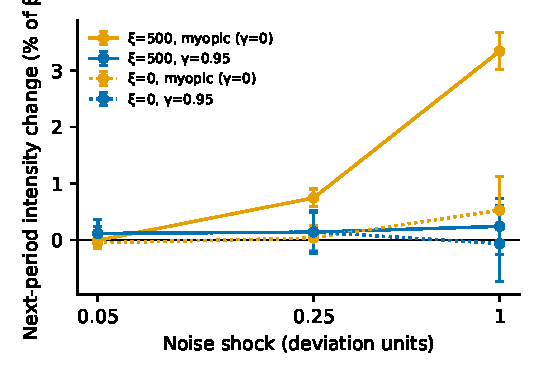
\includegraphics[width=0.5\linewidth]{figures/fig_shared.pdf}
  \caption{Noise-shock responses with shared Q-tables. At $\xi=500$ the myopic
  placebo (orange, solid) ignores small shocks and reacts to large ones, the
  threshold pattern read as a price trigger, although with $\gamma=0$ it has no
  reason to punish.}
  \label{fig:shared}
\end{figure}


\begin{table}[t]
  \centering
  \small
  \resizebox{\linewidth}{!}{\begin{tabular}{llccccc}
\toprule
$\xi$ & Separate Q-tables & $\Delta$ intensity & $\Delta$ profit & Shock response & Rival reaction & Seeds \\
\midrule
0 & $\gamma=0.95$, remembers price & $0.48 \pm 0.00$ & $0.59 \pm 0.04$ & $0.45 \pm 0.58$ & $-0.66 \pm 0.50$ & 1 \\
0 & $\gamma=0$ (myopic placebo) & $0.63 \pm 0.00$ & $0.74 \pm 0.04$ & $0.27 \pm 0.54$ & $0.32 \pm 0.58$ & 1 \\
0 & $\gamma=0.95$, no memory & $0.37 \pm 0.02$ & $0.50 \pm 0.05$ & $0.00 \pm 0.00$ & $0.00 \pm 0.00$ & 1 \\
500 & $\gamma=0.95$, remembers price & $0.48 \pm 0.00$ & $0.63 \pm 0.01$ & $0.14 \pm 0.72$ & $-0.37 \pm 0.86$ & 1 \\
500 & $\gamma=0$ (myopic placebo) & $0.13 \pm 0.00$ & $0.21 \pm 0.01$ & $0.59 \pm 0.40$ & $0.47 \pm 0.46$ & 1 \\
500 & $\gamma=0.95$, no memory & $0.24 \pm 0.02$ & $0.36 \pm 0.03$ & $0.00 \pm 0.00$ & $0.00 \pm 0.00$ & 1 \\
\bottomrule
\end{tabular}}
  \caption{\citet{dou2025} calibration with separate Q-tables
  ($1.5\times10^7$ periods, 100 markets). Shock response: change in
  per-trader intensity one period after a noise shock equal to one
  best-response deviation, as a fraction of $\beta^N$. Rival reaction: change
  in rivals' intensity one period after a forced best-response deviation, as a
  fraction of $\beta^N$. The informativeness index is omitted because at
  $\xi=500$ the Nash and cartel informativeness both equal one to four
  decimals. 95\% CIs.}
  \label{tab:dou}
\end{table}

\begin{figure}[t]
  \centering
  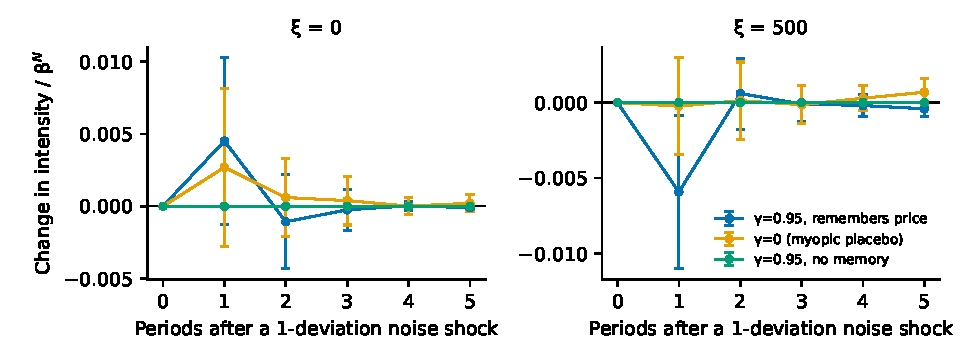
\includegraphics[width=0.9\linewidth]{figures/fig_dou.pdf}
  \caption{Noise-shock impulse responses in the \citet{dou2025} calibration.
  A noise-trader shock equal to one best-response deviation hits at lag 0;
  lines show the change in per-trader intensity relative to $\beta^N$. Under
  price-trigger strategies intensity would jump at lag 1; it does not.}
  \label{fig:dou}
\end{figure}
